\documentclass[10pt,a4paper]{report}
%\usepackage[latin1]{inputenc}
\usepackage[utf8]{inputenc}
\usepackage{amsmath}
\usepackage{amsfonts}
\usepackage{amssymb}
\usepackage{graphicx}
\usepackage{multicol}
\usepackage{tabularx}
\usepackage{tikz}
\usetikzlibrary{arrows,shapes,automata,petri,positioning,calc}
\usepackage{hyperref}
\usepackage{tikz}
\usetikzlibrary{matrix,calc}
\usepackage[margin=0.5in]{geometry}
\providecommand{\norm}[1]{\left\lVert#1\right\rVert}
\providecommand{\sbrak}[1]{\ensuremath{{}\left[#1\right]}}
\providecommand{\lsbrak}[1]{\ensuremath{{}\left[#1\right.}}
\providecommand{\rsbrak}[1]{\ensuremath{{}\left.#1\right]}}
\providecommand{\brak}[1]{\ensuremath{\left(#1\right)}}
\providecommand{\lbrak}[1]{\ensuremath{\left(#1\right.}}
\providecommand{\rbrak}[1]{\ensuremath{\left.#1\right)}}
\providecommand{\cbrak}[1]{\ensuremath{\left\{#1\right\}}}
\providecommand{\lcbrak}[1]{\ensuremath{\left\{#1\right.}}
\providecommand{\rcbrak}[1]{\ensuremath{\left.#1\right\}}}
\newcommand{\myvec}[1]{\ensuremath{\begin{pmatrix}#1\end{pmatrix}}}
\let\vec\mathbf

\newenvironment{Figure}
  {\par\medskip\noindent\minipage{\linewidth}}
  {\endminipage\par\medskip}
\begin{document}
%--------------------logo figure-------------------------%
\begin{figure*}[!tbp]
  \centering
  \begin{minipage}[b]{0.4\textwidth}
    
\includegraphics[scale = 0.05]{iitlogo.jpg}
  \end{minipage}
  \hfill
  \vspace{5mm}\begin{minipage}[b]{0.4\textwidth}
\raggedleft  
\includegraphics[scale = 0.10]{nrc.png}\

  \end{minipage}\vspace{0.2cm}
\end{figure*}
%--------------------name & rollno-----------------------
\raggedright \textbf{Name}:\hspace{1mm} Namrath Pinnamaneni\hspace{3cm} \Large \textbf{Assignment-4}\hspace{2.5cm} % 
\normalsize \textbf{Roll No.} :\hspace{1mm} FWC22042\vspace{1cm}
\begin{multicols}{2}

\raggedright \textbf{Problem Statement:}\vspace{2mm}
\raggedright \\If a line intersects two concentric circles (circles
with the same centre) with centre O at A, B, C and D, prove that AC = DB.
\vspace{5mm}

%----------------figure--------------%
\begin{center}
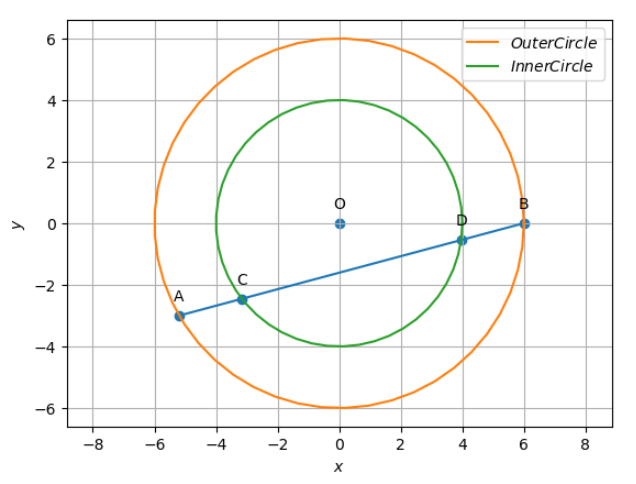
\includegraphics[width=0.5\textwidth]{matrix.png}  
\end{center}\vspace{5mm}
\vspace{2mm}  

%-----------------------------solution---------------------------
\raggedright \textbf{SOLUTION}:\vspace{2mm}\\
Let A and B be the end vertices of the chord intersecting two concentric circles, therefore C and D are points of the chord intersecting inner circle. We solve for the required points C and D as follows.\vspace{4mm}\\

\textbf{STEP-1}\vspace{2mm}\\
Calculating co-ordinates A and B : \vspace{2mm}\\ 
Outer Circle has a radius, $r_o$ = 6\vspace{2mm}\\ 
Inner Circle has a radius, $r_i$ = 4\vspace{2mm}\\
We get coordinates of vertices A and B as follows :\vspace{2mm}\\

\begin{align}
\vec{A} &= r_o\myvec{cos\theta_1 \\ sin\theta_1 }, \vec{B} = r_o\myvec{cos\theta_2  \\ sin\theta_2} 
\end{align}

\vspace{5.2mm} 
By taking $\theta_1 = 159^o$ and $\theta_2=0^o$, \vspace{2mm}\\
We get, 
\begin{align}
\vec{A} &= \myvec{-5.2 \\ -3}, \vec{B} = \myvec{6 \\ 0} 
\end{align}

\textbf{STEP-2}\vspace{2mm}\\
Finding the equation of line AB : \\\vspace{2mm}
Using the parametric equation of the line
		    \begin{align}
			    \label{eq:line-param}
			    \vec{x} &= \vec{A} + \lambda \vec{m}
		    \end{align}
We know the equation of circle is,\\
\begin{center}
    $ x^2 + y^2 = r^2 $ \vspace{2mm}
\end{center}
The above equation can be expressed in vector form as
		    \begin{align}
			    \label{eq:circ-param}
			    \vec{x}^{\top}\vec{x} &= r^2
		    \end{align}
		    
Substituting \textbf{(2)} in above Eq.,
\begin{align}
	\brak{ \vec{A} + \lambda \vec{m}}^{\top}
	\brak{ \vec{A} + \lambda \vec{m}}
	= r^2
\end{align}
\begin{align}
    \implies \lambda^2\norm{\vec{m}}^2+ 2 \lambda \vec{m}^{\top}\vec{A}+\norm{\vec{A}}^2 - r^2 = 0
\end{align}
yielding 
		    {\small
		    \begin{align}
			    \label{eq:cbse-2020-circ_lam}
		\lambda = \frac{-\vec{m}^{\top}\vec{A}\pm \sqrt{\brak{\vec{m}^{\top}\vec{A}}^2 -\norm{\vec{m}}^2\brak{\norm{\vec{A}}^2 - r^2 }}}{\norm{\vec{m}}^2}
		    \end{align}
		    }
For this problem, the numerical values are
\begin{align}
\vec{A} &= \myvec{-5.2 \\ -3}, r = 4, 
\end{align}
\begin{align}
\vec{m} = \vec{B} - \vec{A}, \vec{m} &= \myvec{11.2 \\ 3}
\end{align}

Substituting above in \textbf{(6)},
\begin{align}
\lambda_1 = 0.18, \lambda_2 = 0.82
\end{align}

Thus substituting $\lambda_1$ and $\lambda_2$ in {\textbf{(2)}} would give the desired points of intersection C and D.\vspace{2mm}\\

For point C,
\begin{align}
\vec{x} &= \myvec{-5.2 \\ -3} +  \lambda_1 \myvec{11.2 \\ 3}
\\
&= \myvec{-3.16 \\ -2.45}
\end{align}

For point D,
\begin{align}
\vec{x} &= \myvec{-5.2 \\ -3} +  \lambda_2 \myvec{11.2 \\ 3}
\\
&= \myvec{3.96 \\ -0.55}
\end{align}
Thus, points C and D
\begin{align}
\vec{C} &= \myvec{-3.16 \\ -2.45}, \vec{D} = \myvec{3.96 \\ -0.55} 
\end{align}

\textbf{Table} \vspace{2mm} \\

The input parameters are the lengths points A and C. \vspace{2mm} \\
{
\setlength\extrarowheight{2pt}
\begin{tabular}{|c|c|c|}
	\hline
	\textbf{Symbol}&\textbf{Value}&\textbf{Description}\\
	\hline
	$r_o$ & 6 &Outer Radius\\
	\hline
	$r_i$ & 4 & Inner Radius\\
	\hline
	\textbf{m} &$
	\begin{pmatrix}
		11.2\\
		3\\
	\end{pmatrix}$
	& Direction Vector of the Line\\
	\hline
\end{tabular}
}\vspace{6mm} \\
\textbf{Construction} \vspace{3mm} \\
{
\setlength\extrarowheight{2pt}
\begin{tabular}{|c|c|}
	\hline
	\textbf{Vertex}&\textbf{Co-ordinates}\\
	\hline
	O & (0,0)\\
	\hline
	A & (-5.2,-3)\\
	\hline
	B & (6,0)\\
	\hline
	C & (-3.16,-2.45)\\
	\hline
	D & (3.96,-0.55)\\
	\hline
\end{tabular}
}

  \end{multicols}
\end{document}
